Notizen zur Entwicklung mit Flutter:
\TODO{https://www.youtube.com/watch?v=wE7khGHVkYY}
Composition: Composing different existing widgets to a new one

Durch voreinstellung und Erstellen eines Basic screen schon nach wenigen Minuten eine erste laufende "Version" zu sehen.

Hot Reload zeigt sofort sichtbare Änderungen, so dass man gut UI debuggen umbauen und anpassen kann.

Schwer herauszufinden welche Elemente es gibt, wie man sachen konfigurieren kann. Am Anfang nicht sehr intuitiv. Man muss sich auf jeden Fall gut in die Doku einlesen und vlt. auch ein kleines Tutorial machen, bzw. die genauen Sachen googlen.



\section{Flutter 101}
\subsection{Widgets}
Widgets sind die Elemente in Flutter, die genutzt werden um die Applikation aufzubauen.
Es gibt zwei Arten von Widgets:
1. Statefull Widget
2. Stateless Widget
Der Unterschied ist, dass bei Statefull widgets, gibt es noch eine State Klasse, die den aktuellen Status des Elements speichert und bei einer Änderung die neuen Werte übernimmt und damit eine Änderung in dem Element ausführt. Am besten ist dies etwa mit einem Favoriten Button vorstellbar. Drückt man ihn, fügt man ihn zu den eigenen Favoriten hinzu und das Icon des Buttons ändert sich bspw. von einem Herzicon, das nur den Rahmen hat, zu einem was ausgefüllt ist.

Bei der Erstellung gibt es einiges zu beachten. 
Etwa kann man auch ein Widget erstellen wollen, dass in ein eigenes File auslagern, wie es mit tobBar.dart ist. Hier ist jedoch dann die übergabe von Parametern wieder wie bei normalen Klassen übergeben werden. Man kann sie aber auch erstellen wie bei topBar2.dart, wo man die einzelnen Parameter bennenen kann und auch besser nullabillity handln kann.
\TODO{genauer untersuchen. Vorallem Statless Widgets, nullability wie bei topBar, und vieles mehr}

Man kann aber auf jeden Fall sehr einfach ein eigenes Widget schreiben. Dies ist vorallem sinvoll, wenn man eine Komponente hat, die man wiederverwenden möchte. Man erstellt einfach die Widgetclasse mit den entsprechenden 
\subsection{Plugins, Modules, Packages}
Im Verlauf der Arbeit wurde ebenfalls Testweise ein eigenes Plugin geschrieben um zu testen wie hier der entsprechende Ablauf ist, und wie hiermit eventuelle nicht vorhandene Funktionalität mit nativen Programmiersprachen und API calls programmiert werden kann. Hierzu wurde einmal die Einführung von der google developer seite TODO: Link genutzt um ein iOS und Android keyboard zu schreiben das auf dem Gerät anhand von nativen APIs der Betriebssysteme die Töne erzeugt und dabei sowohl auf drauf drücken und loslassen reagiert.
Das interessante an dieser Methode ist es , dass zur Kommunikation zwischen dem Dart Code und dem nativen Code channels zur Kommunikation genutzt werden, um dann die entsprechende native Funktionalität auszuführen. Ein zweiter interessanter Punkt ist, dass plugins asynchron auf eigenen Threads ausgeführt werden/können. Dies folgt der größeren Diurektive dass UI und Logik auf unterschiedlichen Threads laufen, um mögliche Blockaden nicht auf dem jeweils anderen Thread bem,erkbar zu machen.



\subsection{Layout}
-Button
-Row
-Wrap
-Container: Dies ist das Wichtigste Widget von Flutter. Sobald man irgendwelche Platzhalter oder innere Abordnung oder sonst was nötig ist, braucht man oftmals das Widget Container. Man kann ganz einfach andere Elemente in ein Container hineinstecken und alle benötigten Sachen hinzufügen. Von Margin Paddings feste Größen und vieles mehr. Einfach Einen Container erstelle und die innenliegenden Elemente in einem ChildWidget hinzufügen.
-Scaffold
\subsection{Aufbau}
-Widgets
-classes
-Stateclasses
-Navigator / Router
-Assets

\subsection{Plugins / pubspec.yaml}
\subsubsection{benutzte Plugins}
\subsubsection{Lehre aus Unterhaltung mit Entwicklern von Plugins}
Bei erstellen erster Seiten und hinzufügen ersten Packages Fehler aufgetreten betreffend Not implemented. Fehlermeldung und Fehler-stack nicht sehr aussagekräftig. Wurde evaluiert dass es an simple gradient text lag. Laut Dokumentationseite des Packages ist es kompatibel für alle Plattformen. Jedoch funtkionierte es nach hinzufügen der Vorgeschlagenen Lösung nur noch auf Android/mobile. Beim Nachforschen tut man sich schwer genaue Gründe herraus zu finden, da die Fehlermeldung und die Dokumentation hierfür leider keinerlei Hinweise gibt. 
Es kam im Verlaufe der Fehlererforschung auch zum Kontakt mit dem Entwickler der sehr hilfsbereit die Fehlerforschung unterstütze.
\TODO{Ergebniss der Issueunterhaltung mit Entwickler}
Bei genauer untersuchung mit dem Entwickler zusammen kam herraus, dass meine Flutterversion eine ältere war, als die, die benötigt wurde, um das Plugin auf Web laufen zu lassen. Nachdem die Flutter version angepasst war, funktionierte es einwandfrei. Da es jedoch bei vielen Packages und auch bei diesem keine Angaben zur mindestens zu nutzenden Flutterversion gab, empfohl ich dem Entwickler doch dies in der Read.me hinzuzufügen, was auch prompt geschah. 
An diesem Beispiel sieht man sehr gut, dass diese Community sehr aktiv und offen ist für Vorschläge und Veränderungen.
Es hat mir jedoch auch gezeigt, dass einige Sachen hier Fehlen:
1. Eine Angabe welche Flutterversion genutzt werden muss, damit alles gut funktioniert. Es gibt zwar eine Angabe unter welcher Version das Plugin getestet wurde, aber manchmal will man vlt. gar nicht sofort auf die neueste Version wechseln.
2. Eine Anzeige welche Packete und Flutterversionen geupgraded werden können, fehlen. Es muss irgendein Anhaltspunkt geben um schnell zu sehen, welche Plugins bzw. Dependencies veraltet sind und was hier geupdated werden kann.


\section{Layouting in Flutter}
SpacerFürTODO
\TODO{Eigentlich hat ja android das auch. Hier sind halt die Layout Files wirklich nur } 
\TODO{reine Layout Files aber sie sind ja auch xml. Siehe vergleich mit HTML+CSS} 
Flutter ist ersteinmal etwas anderes als die native Entwicklung. 
\TODO{Mit iOS abgleichen}
Containerisierter Aufbau Abgleich miut Kapitel zu Layout aus der Flutter - Doku

Flutter ist ähnlich zu html+css Aufbau Man verschachtelt die verschiedenen Elemente ineinander um dann einen Container-Baum zu erhalten.
Dies ist sehr ähnlich zum html baum. Der entsteht wenn man eine Website entwirft und die verschiedenen Elemente verschachtelt. 
Allerdings kommt hier auch gleich noch css mit rein, da man die verschiedenen Attribute der Elemeente direkt beschreibt.
Was anders ist, ist dass man für Layout spezifische Sachen manchmal noch einen Container braucht, während man ja etwa margin auf jedes Element drauf machen kann. Es ist aber dementsprechend auch wieder ähnlich, da etwa flex boxen manchmal in sogenannte divs eingebaut werden müssen, um zu funtktionieren. Was außerdem besonders ist, ist dass es schon sehr vordefinierte Plugins gibt, die das Layout vorgeben können. Einerseits gibt es rows und Columns, die ansonsten oft über divs mit bestimmten Klassen und Frontend UI Framewortks erreichrt werden können und es gibt oft auch schon spezifizierte Sachen für Buttons etwa. Hier kann man dann OutlinedButton, Button, TextButton oder auch IconButton nehmen um das Design hierfür nicht erst selber bauen zu müssen.

\begin{figure}[ht]
  \centering
  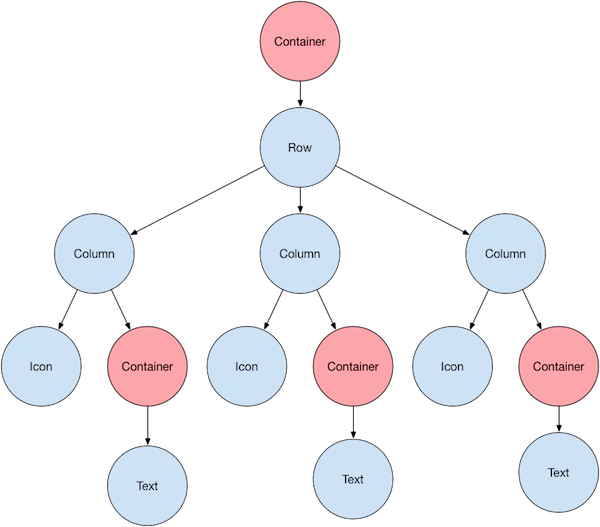
\includegraphics[height=7cm,keepaspectratio]{images/sample-flutter-layout.png} 
  \caption{Hierachie einer Menüleiste Quelle: Flutter Doku}
  \label{fig:flutter_layout_tree}
\end{figure}

Abbildung \ref{fig:flutter_layout_tree}

Um Seiten zu erstellen gibt es verschiedene Methoden. Oft muss man die Seiten komplett selbst aufbauen. Das heißt man fängt beim Startelement an. Dem sogennanten Scaffold. Dieser hat verschiedene Elemente. So gibt es AppBar man kann einen Footer hinzufügen und vorallem gibt es einen Body. Der kann dann ein Widget als Child hinzugefügt werden. Hier kann nun über verschiedene Widgets wieder neue Sachen hinzugefügt werden und so Stück für Stück ein Layout gebaut werden. 
Hierfür gibt es Grundsätzlich zwei verschiedene Arten von Widgets. 
1. Widgets die Helfen die Seite zu strukturieren und Layouts zu verfeinern und aufzubauen.
2. Widgets die Teil der Nutzeroberfläche sind und die unter Umständen noch weitere Childs zur ausgestaltung Besitzen, aber auf der Oberfläche angezeigt werden. So hat etwa ein TextButton noch ein Child Text wo dann der Text hinzugefügt wird, der im Button steht. Der Button ist allerdings ebenfalls ein Teil der UI. Anders als Container. Diese fügen eventuell eine Margin, also Abstand zu anderen Elementen hinzu oder ändern\TODO{Tun sie das wirklich?} unter Umständen auch mal den Hintergrund, sie sind allerdings keine Alleinstehenden Elemente und umgeben eigentlich nur das Child oder die Child Elemente.




\section{Conclusion Flutter}
Hier auf die Challanges mit Null safety und grundsätzlichen Änderungen zwischen den großen Versionen eingehen, die dazu führen, dass nicht nur unter anderem auch eigene Dokumentation und Codelabs Einträge nicht mehr funktionieren, sondern auch ein großteil der bestehenden Lösungen so nicht mehr einfach Copy Paste mäßig in die eigene Applikation gezogen werden kann.
Dazu kommt, dass etwa reihenweiße Packages mit einem Update auf Flutter 3.0 wieder ein Update brauchen da hier wieder einige Sachen zu Nullsafety usw. siehe Screenshot mit Warnung aus Console und der Nutzer dann immer eine Warning bekommt, die er so schnell nicht ändern kann. Dazu kommt, dass das upgraden der Dependencys wie bei allen anderem aber auch, wieder zu häufigen Koabhängigkeiten und Upgrade Issues führt, sodass man immer genau aufpassen muss, ob man denn jetzt eine ältere bzw. neuere Version der Plugins nutzen kann. Deswegen gilt auch hier wie in vielem anderen. Versuche so viel wie möglich selbst zu machen. Hierzu vlt. aus dem Artikel zietieren mit jeder Import ist ein "Dept" und irgendwann muss man dann seine Schulden zurückzahlen. Natürlich gilt. Nur so viel wie sinnvoll. Denn man sollte bereits verfügbare Lösungen zu komplexen Problemen schon nutzen, um nicht unnötig Zeit zu verschwenden. jedoch sollte man hier darauf achten, dass man vlt. nur so viel importiert wie nötig ist, um möglich Cropssdependencie errors zu vermeiden.
Ein weiterer Punkt ist die verfügbarkeit auf Plattformen. Nachdem mit Flutter 3 die Lücke der letzten Fehlenden Plattformen geschlossen wurde, heißt es nicht dass man jetzt einfach seine für Android und iOS entwickelte App nehmen kann und dann eine Plattform hinzufügen und dann der Meinung sein dass alles einfach funktioniert. Denn einige Plugins sind nur für bestimmte Plattformen geschrieben. So etwa das WebView Plugin für Flutter. Die populärste von Flutter "promoted(noch mal nachschauen)" Version ist nur für Android und iOS. Das ist ja eigentlich auch erst mal ok, da man ja bei allen anderne Versionen einfach eine Website aufrufen kann und dabei auch keine Layout probleme haben sollte. Aber wenn man sich vornimmt nun für eine andere PLattform eine App mit WebView zu bauen, so hat man leider nie das alles in einem Paket. So gibt es Plugins die unterstützen dann zusätzlich noch Windows Version oder die Webversion, oder eine andere die alle Laptop Plattformen (Mac, Linux, Windows) unterstützt, aber dann wieder nciht die Smatrphone Versionen. Hier muss man also bei Projektbeginn sich überlegen, für welche Plattformen man etwas entwickeln will, bzw. welche Plattformen man ausschließen kann und dann dementsprechen deine Plugins suchen, was eiunen auch stark einschränken kann. Natürlich gibt es jetzt die Möglichkeit einfach sein eigenes Plugin zu schreiben und dabei alle Plattformen zu unterstützen. Dafür muss man sich jedoch dann auch in jeder zu unterstützenden Plattformtypischen Programmiersprache auskennen.